%************************************************
\chapter{Automatic programming}\label{ch:code-gen}
%************************************************

\begin{flushright}{\slshape Writing machine code involved several tedious steps—breaking down a process into discrete instructions, assigning specific memory locations to all the commands, and managing the I/O buffers. [...] We needed to understand how we might reuse tested code and have the machine help in programming. [...] This led to the development of interpreters, assemblers, compilers, and generators—programs designed to operate on or produce other programs, that is, automatic programming.} \\ \medskip
    --- Mildred ``Milly'' Kross
\end{flushright}

Creating a computer program is a challenging and engaging experience, it requires expertise, brilliance and ingenuity. At the same time, writing code is a mundane and dull activity, it requires to complete repetitive tasks, to manage multiple small issues and to deal with problems unrelated with the main project.

Thankfully, today, we are not dealing with the same difficulties that Mildred Kross faced when working on the UNIVAC I. Multiple technological advancements and progresses in Computer Science gave us compilers, high-level programming languages, design paradigms, frameworks, middleware, integrated development environments, and more. All these tools exist to make computer programming more about designing and developing a program than writing code. 

During Computer Science history, the concept of automatic programming changed to adapt to the expectation of the time. Originally, it was the automation of the process of punching paper tape, later it became the transformation of high-level programming languages (\eg, Fortran and ALGOL) to machine code, a task that, nowadays, is integral part of the build process. Today, automatic programming mostly refers to the automatic generation of executable code from representations that are not programming languages. These representation may have different level of abstraction, from the closest to the target (\eg, domain specific languages, flowcharts, \etc) to the furthest (\eg, graphical representations, models, \etc).

%TODO complete after the end of the chapter
This chapter presents our approach to automatically generate ROS code from the AADL model.

\minitoc
\newpage

\begin{figure}[t]
    \centering
    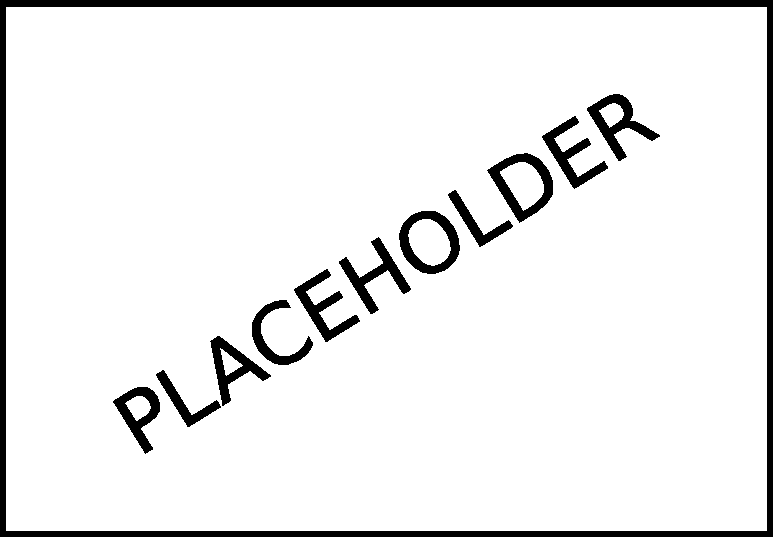
\includegraphics[width=0.8\textwidth]{gfx/placeholder}
    \caption{TODO}\label{fig:code-gen}
\end{figure}

\section{Generating ROS artefacts}
An automatic programming approach is a collection of rules and methods to transform an initial description to a different, more complex output. Therefore, even before the definition of the transformation itself it is necessary to define the input and the output of the process. In Chapter~\ref{ch:Modelling} we described in details a collection of meta-models that can be used to define ROS architectures using AADL in combination with a data modelling language (\ie, ANS.1 or JSON schema). A model compatible with this meta-models is the starting point of our automatic code generation process. Since the expected output of the entire process is a complete working architecture, the model alone is not enough as an input. To have a functioning architecture, the designer needs to pair the model definition with the implementation of the node inner functionalities; this can be done by using AADL properties. A ROS complete architecture is composed by multiple elements: existing nodes run as external resources, new nodes and messages created by the developers, launch files to organize the architecture, parameter profiles to configure the system. All these elements are  captured by the model, and can be automatically generated by our process. First, the automatic programming system creates the source code for the new custom nodes, the target language is C++. ROS supports multiple languages, mainly C++ and Python, Lisp is officially supported but rarely used, and there are experimental libraries for Java and Lua. From the ROSwiki, \textit{rospy} (\ie, the Python implementation of ROS) is suggested as the approach that promotes implementation speed (\ie, reduced development time) over runtime performance, and it is designed specifically for fast prototyping, testing and lightweight implementations (\eg, configurations and initialisations), while \textit{roscpp} (\ie, the C++ implementation of ROS) is considered the main library, and it is designed with a focus on high performances and runtime speed. Since the output of the automatic programming is at the end of a long process of design and development of the architecture, we decided to use \textit{roscpp}, and therefore C++, as the target library to achieve the most efficient and robust implementation. Since C++ is a compiled language, the system will automatically generate all the necessary files to build the node executable, if the designer specify all the necessary information in the model (\ie, source code of the functionalities), the final output of the automatic programming process will be ready to compile with no intervention required. The automatically generated code will be placed in the correct package structure expected by ROS, together with any custom message, service or action file. This covers everything necessary for the execution of single nodes, to put them together in an architecture it is necessary to create launch files. In launch files, the designer specifies the instances of the nodes and how they are connected, by renaming all the necessary topics, and configured, by including configuration files. The topology of the architecture can be automatically extracted from the model and converted in a launch files, and the parametrisation defined using a data modelling language (\ie, ANS.1 or JSON schema) can be converted in the YAML description used by ROS. Moreover, in launch files existing nodes are included in the architecture and connected to the rest of the topology.

Figure~\ref{fig:code-gen} summarises the complete process. Our automatic programming approach requires as input a model defined in AADL, completed by a data description using ASN.1 or JSON schema, and specialised via properties to include functionality-specific source code. When all these conditions are met, the process provides as an output a collection of automatically generated and compilation-ready ROS nodes, their associated communication files (\ie, messages, service and action files) and the necessary launch files to run the architecture. A fully complete model creates and architecture that only needs to be compiled and run.

\begin{figure}[t]
    \centering
    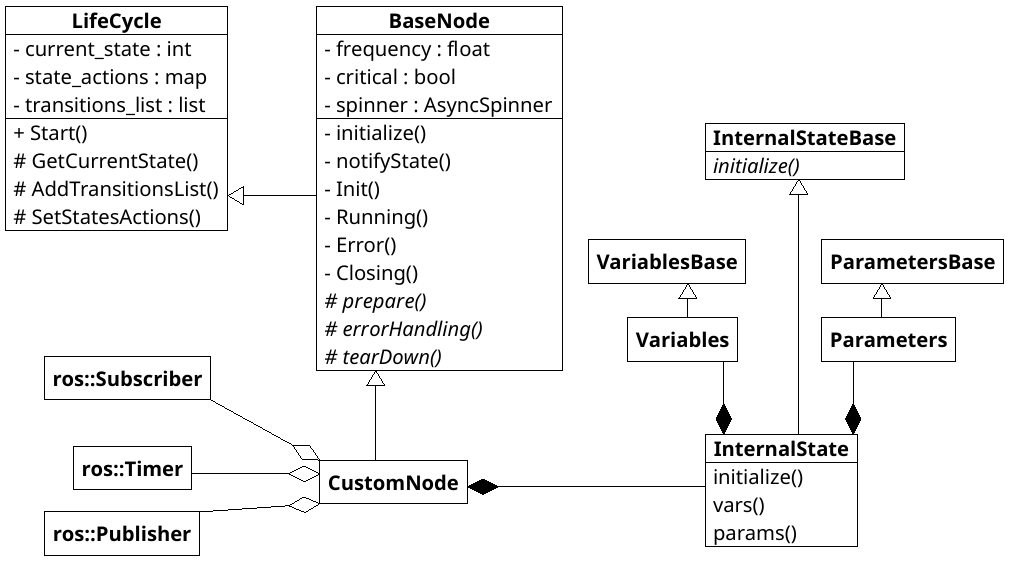
\includegraphics[width=\textwidth]{gfx/class}
    \caption{TODO}\label{fig:node-class}
\end{figure}

\section{Engineered ROS node}
\label{sec:ros-node}
Differently from other middleware or frameworks, ROS does not constrain the developer on the structure of the components; it was designed to be maximally flexible following the mantra: ``\textit{we don't wrap your main()}''. While this approach certainly contributed to the popularity and growth of ROS as a middleware and de facto standard for robotics, at the same time it created a very heterogeneous landscape for ROS nodes. Some of them are well designed, rich in functionalities, robust and configurable, others are cobbled together for a prototype and then used as legacy code for one single core functionality. Often this second category is created by experts in a specific field (\eg, vision, control, manipulation, \etc) that lack the necessary programming and software engineering skills and knowledge to develop a well-designed and robust node. With our approach we are targeting specifically this category of developers, that posses the expertise to contribute to the robotic community, but are discouraged by the programming required.

Since ROS does not impose any structure for the node, the simplest approach for automatic code generation would be to target an essential node, covering the minimum functionalities required to run it. There are few advantages in this approach: easier to implement code generator, simpler and more readable output, an implementation closer to what the developer knows. However, such a direct approach would have significant downsides: a lax relationship between the node and its model, lack of advanced functionalities that can be hidden in the automatic programming approach, less flexibility of the implemented node, more work left to the developer (\eg, testing, debugging, performance evaluation, \etc), more tampering by the developer with the basic structure of the node, no real benefit between a handcrafted and an automatically generated node. For all these reasons we decided to created a engineered base node that can be used as a reference and starting point for automatic code generation.

%TODO may not be simplified in the final version
Figure~\ref{fig:node-class} shows a simplified UML diagram of a custom node based on the engineered ROS node. Immediately, it is possible to recognise three main components: \textit{LifeCycle}, \textit{ROSNode}, and \textit{InternalState}. Each of them represent one of the main characteristics captured by the engineered node. The \textit{LifeCycle} implements an internal state machine that controls the evolution of the node. The \textit{ROSNode} is the core implementation of the node, capture all the ROS-related functionalities and management procedures. The \textit{InternalState} capture all the developer-defined parameters and variables necessary for the correct execution of the node.

\subsection{Life cycle}
When working with component-based approaches, it is important to define a recurring and consistent behaviour of a component, in the case of robotic components it is even more important, since they often operate in time and functionality critical condition. In Section~\ref{sec:ros-in-aadl}, we presented how a life cycle of a node can be modelled in AADL, and how it can be used to guide the initialisation, configuration and execution of a component. To capture the same behaviour in the engineered node, we developed the \textit{LifeCycle} class to define the evolution of the node. While various implementations of state machines in C++ already exists, a very popular one has been around for almost 20 years\footnote{https://www.codeproject.com/Articles/1087619/State-Machine-Design-in-Cplusplus-2}, we opted to create a stripped down version that trades some functionalities for simplicity, understandability, and modern development approaches. The result is a very lightweight state machine, that supports dynamically defined states and transitions and it is completely ROS-independent.

To maintain the generality of the implementation, the class itself does not specify any state or transition. It only defines an empty enumeration that the subsequent classes can extend to define their own states. The valid transitions are defined as a list of pairs, going from one state to another, as for the states, the list is created by classes extending or using the state machine. The last initialisation step before running the state machine is to bind each state with a function. In practice, the binding is done by creating a map with the state as the key and an \texttt{std::fuction} as the value. Class template \texttt{std::function} is a general-purpose polymorphic function wrapper, it can be assigned to any callable target (\eg, functions, lambda expressions, pointers to member functions, \etc), this makes this approach particularly flexible and not bound to any specific implementation. When the initialisation is complete, the state machine can be started, the initial state is the one defined in the constructor, but there is no specific definition for a termination state. At each execution loop, first, the state machine execute the function bound to the specific state, then, it checks if there is a valid transition waiting to be performed, if there is one, the loop repeats and a new state-bound function is executed, otherwise the state machine has reached a final state and the execution terminates. While the list of all possible transitions is defined during the initialisation phase, each specific change of state is defined at runtime in all the state-bound functions. This is necessary, for example, to distinguish between a successful component initialisation that goes from an initial to a running state, to an unsuccessful one that would take the component to an error state. In practise, at the end of each state-bound function, the developer needs to specify the next state depending on the current state of the execution, then the state machine will check if the transition is valid (\ie, it is in the transitions list) and execute it. Mirroring the model presented in Section~\ref{sec:ros-in-aadl}, the engineered node supports five different states: initialisation, running, error report and closing. How they are implemented, what is their role and which ROS functionalities they evoke will be detailed in the next section.

\begin{figure}[t]
    \centering
    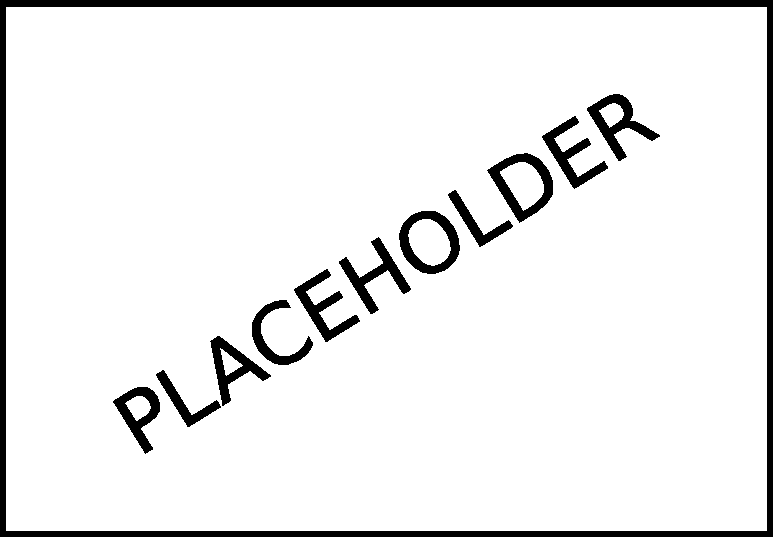
\includegraphics[width=0.8\textwidth]{gfx/placeholder}
    \caption{TODO}\label{fig:state-machine}
\end{figure}

\subsection{ROS node}
The core implementation of the engineered ROS node is in the \textit{ROSNode} class, here the life cycle is defined and materialised, and all the basic ROS-related functionalities are implemented. By defining this class, we can streamline the development process of a component by hiding the base initialisation procedure of a ROS node, create a well defined structure the developer can follow, and enhance the base implementation by adding additional functionalities (\eg, error detection and state report). The \textit{ROSNode} class extends directly the \textit{LifeCycle} class, therefore, the first implementation step is to define the states, the valid transitions and method bound to each state. Figure~\ref{fig:state-machine} presents the complete definition of the internal state machine, this mirrors the description provided in Section~\ref{sec:ros-in-aadl}. Each state is bound to a specific method of the class, and it implements a core functionality of the node.

\paragraph{Init} This method is bound to the initial state of the node (\ie, \texttt{ST\_INIT}). It is defined as a two-steps process and all the initialisation procedures of the component are implemented here.

The first step is a common initialisation that applies to every node, it sets up the ROS environment and defines the asynchronous spinner\footnote{http://wiki.ros.org/roscpp/Overview/Callbacks and Spinning}. In Section~\ref{sec:ros-in-aadl}, we modelled the ROS node with a external port to communicate the current state of the node after every transition, in this phase of the initialisation, the base node create the connection with the ROS service in charge of receiving this notifications. In ROS, a client can register to a service even if the server is not active, all the communications are lost until the service is finally started. This behaviour is not a problem for a status notification system, since it is meant to exist only to supervise the general evolution of the internal life cycle of the node. Nevertheless, our aim is to create a flexible base node that can adapt to different situations, thus, we defined an extra configuration property for the node, the developer can initialise the node as \textit{critical}. When a node is critical, instead of just starting the status notification service, the initialisation procedure will wait until the service is up, and then registers to it. In this way, an external supervisor node in charge of monitoring all the critical nodes can trace the entire evolution of their life cycles and act accordingly if something does not behave as expected. After the general initialisation procedure, the first action is to externally notify the state of the node, again the notification method itself behave in a different way for critical and non-critical nodes. To save bandwidth and reduce the number of requests, non-critical nodes notify their new state after a transition only if it is different from the previous one, in other words, they do not notify transitions on self-loops. Critical nodes are meant to be constantly monitored by the supervisor, therefore they notify their state after every transition, basically, in this case, self-loops are used as a way to measure the liveness of the node.

If the basic initialisation is completed successfully, the second step of the set up of the node is activated. An unsuccessful outcome is considered a critical failure and the node is instantly shut down. The second part of the initialisation is an abstract method not implemented in the \textit{ROSNode} class (\ie, the \textit{prepare} method) and it is meant to be used by the child class to define any node-specific initialization procedures. The developer can use this method to fill parameters and variables with their initial values, set up publishers and subscribers, or perform any other special initialisation (\eg, activate hardware connections, pre-fill data structures, \etc). If this preparation phase is completed successfully the method will trigger the transition to the main execution state. Differently from the base initialisation, an unsuccessful preparation phase will trigger a transition in error state. This is because we cannot anticipate what kind of procedure the developer will implement in this second part of the initialisation, therefore issues in these phase may be resolved in a specific error management procedure and lead to a successful initialisation.

\paragraph{Running} A complete and successful initialisation will transition the state machine in the \texttt{ST\_RUNNING} state, and this is the method bound to it. Since the engineered ROS node is built around an asynchronous spinner, most of the ROS-related functionalities (\ie, checking subscribers, services and timers) are executed in a separate thread, hence this method only needs to check for errors or node termination. When the node is working with no issues, the \textit{Running} method is just a low-frequency (\ie, 1 Hz) repeating self loop, two things can change this status quo: first, one of the asynchronous activities (\eg, a subscriber callback) sets an error flag, or second, an external signal triggers the shutdown procedure. In the former case, this method interrupts its self loop and trigger a transition to the error state, in the latter, it receives the signal and changes the current state of the life cycle to shutdown. When the node is initialised as \textit{critical}, the behaviour of the \textit{Running} method does not change, however, the state notification happens at every self loop instead of only after the first transition. Given the fundamental functionalities implemented in this method, the developer cannot directly modify it, however it is possible to change the frequency of the self loop. Given the structure based on the asynchronous spinner, changing the frequency will not influence the behaviour of any ROS-related functionality, but it can change how fast the node reacts to errors or terminations; specifically, the higher the frequency the shortest will be the time between the generation of errors and interrupts and their detection. Changing the frequency of the self loop it is also useful to monitor the liveness of critical nodes. 

\paragraph{Closing} As any other process, ROS nodes can be closed by sending a termination signal (\ie, SIGINT). Normally, they already implement a handle to capture the signal and force a shutdown of the node, in the engineered node we replace it with our own version. Our handle does not perform any shutdown procedure, it just capture the signal and sets a flag; this flag will cause the \textit{Running} method to trigger a transition to the \texttt{ST\_CLOSING} state.  In this method bound to the state is where the actual shutdown procedure happens: first, it triggers a final state notification, so a potential supervisor knows that the node is shutting down, then it execute a custom \textit{tearDown} method, and finally it shuts down any ROS-related functionality. The \textit{tearDown} method is the shutdown counterpart of the \textit{prepare} method of the initialisation. It is abstract and not implemented in the base class, any child class extending \textit{ROSNode} will implement it with their own specific shutdown procedure. This is down to let the developers gracefully close existing connections (\eg, device drivers), propagate the shutdown to other nodes (\eg, critically dependant components), or provide additional shutdown notifications (\eg, specific logging systems). Since this is the terminal state of the life cycle, this method does not implement any transition.

\paragraph{Error} Natively, ROS does not provides any system to manage errors during the execution of the node. In our engineered node, we created an extensible structure to identify, detect and react to errors. The \textit{ROSNode} class defines an enumeration with few predefined error codes, they cover some common issue that may happen during the normal functioning of a node. They are:
\begin{itemize}
\item \texttt{PARAM\_ERROR}: this is a typical initialisation error, when a necessary parameter is not found in the parameter server. The node cannot run correctly when partially initialised, a way to handle this error is to wait until the parameter is available and then restart the initialisation procedure.
\item \texttt{SUB\_FAILED}: one of the subscribers of the node fails. This may compromise the entire node (\eg, set-point subscriber for a control node) or just disable one of its functionalities (\eg, a multiplexer missing one of the inputs). Depending on the situation this may or may not require the shutdown of the node. 
\item \texttt{PUB\_FAILED}: one of the publishers of the node fails. As for the subscribers, this may be very impactful (\eg, a planner that cannot publish the result) or a minor inconvenience (\eg, a visualisation topic not initialised), and therefore could prompt a shutdown of the node.
\item \texttt{INVALID\_MESSAGE}: This is an error that can be triggered during a subscriber callback or before publishing a message. A message has an unexpected value (\eg, negative distance, out of bound acceleration, empty path). Sometimes malformed messages are inconsequential, and the error handler will just record them, in other cases they can be hazardous and require to halt the node execution. 
\end{itemize}

These error codes are mostly related to the correct execution of ROS functionalities, on top of these, the developer can extend the enumeration and define his own error codes, to cover problem-related corner cases. 

At any moment during the normal execution of the node, the developer can use the \textit{faultDetected} method to notify one of the possible error codes. After the initialisation process or during the \textit{Running} self loop, if any error code is set, the system will transition to the  \texttt{ST\_ERROR} state. The \textit{Error} method is bound to this state, during its execution, first it notifies the state transition, to let any potential supervisor know that the node is in an error state, then it calls a method to handle the error, finally, after \textit{errorHandling} returns, if the error code is still set, the error is unsolvable and the node transition to the \texttt{ST\_CLOSING} state, otherwise, the node can go back to normal execution. The \textit{errorHandling} method is similar to the abstract method used during the initialisation and closing phases, as before, it is an abstract method that the developer can extend in the child class to manage any specifically defined error codes. Differently from the previous two, it is not a pure abstract method, since we provide a basic implementation in the \textit{ROSNode} class to manage the four already defined error codes. The developer can decide to reimplement completely the method (\eg, complex nodes with articulated initialisation procedures), run it alongside the existing one (\eg, few problem-related corner cases), or skip error management and leave only the already defined implementation (\eg, simple node requiring minimal definitions).

\subsection{Internal state}
Components are meant to be reusable through composition and parametrisation. The computation graph of ROS combined with our model-based approach ensure the composability, by providing deployment-time rewiring and decomposing components functionalities. On the contrary, parametrisation is not embedded in the design of the nodes. ROS provides various system-level tools to manage parameters: a centralised system to store and collect parameters (\ie, the parameter server), the corresponding APIs to fetch and set them, and a system to dynamically change parameters in real time. However, how to integrate them in the component is left to the developer. The result is parametrisation is often ignored or misused. Parameters are uncategorised and mixed between functionalities, modified during execution creating inconsistencies, defined conceptually but then hard-coded as constants in the implementation. This issues prompted us, originally, to exploit data modelling languages to capture the parametrisation of the component, and, in the engineered node, to design a separate class to encapsulate the parameters of the node.

Parameters are the external-facing part of the internal state of the component, they codify a specific configuration defined before execution; variables, on the opposite, are internal-facing, they evolve with the node and exist only in the time frame of its execution. As mentioned at the beginning of this section, ROS does not provide any structure to support the implementation of the node, in the case of the variables, it means there is no predefined way to safely store and share between callbacks the information extracted and derived from messages. Normally, there are two approaches used when developing ROS nodes, one is for traditional imperative implementations, where variables are declared as global and shared between callbacks, the other wrap the entire node in a class and uses methods as callbacks and attributes for variables. While this approaches are not inherently wrong, they have significant downsides. They reduce the portability of the design of the node by removing the distinction between ROS-specific (\eg, declaration of publishers and subscribers) and problem-specific (\ie, the necessary logic to implement the functionalities of the node) implementations, they are harder to debug since they are not encapsulated and may have unpredictable side effects, they are more difficult to extend and modify since they do not present a common interface. Our solution is to create an overarching class encapsulating both parameters and variables, and present a single interface that the developer can use to access, modify, share and store the internal state of the component.

As visible from Figure~\ref{fig:node-class}, the internal state of the node is built using a hierarchical approach. The superclass is called \textit{InternalStateBase}, it has two members: a structure for variables of type \textit{VariablesBase} and a constant structure for parameters of type  \textit{ParametersBase}. Parameters are defined as constant, this means that after setting their values during the initialisation phase, it is guaranteed they will not change. An exception to this is when the node implements a dynamic reconfigure system, in this case there is a special callback in charge of managing the parameters and changing them according to an external control panel. In general, by defining the structure as constant it is possible to limit any modification of the parameters to specific procedures, and avoid unintentional modifications using compile-time checks. Both the parameters and variables structures are defined as shared pointers, this pointer-based declaration gives us the ability to treat each structure as a single entity, while, at the same time, avoiding useless and memory-consuming copies when using them in external procedures. The superclass has only one method, an pure abstract initialisation method that the developer has to implement in the child class; this is designed to force the developer to initialise all the parameters in the same location and to set an initial value to all the variables. To increase the flexibility of the base node, the internal state is not declared directly in the \textit{ROSNode} superclass, the developer can extend \textit{InternalStateBase} to create his own internal state class and declare it in the custom node. To better exploit the structure provided by the superclass, the developer can extend the parameters and variables structures, to define all the problem-specific details.

\section{Custom ROS node}
In Section~\ref{sec:ros-node}, we presented the engineered node as the starting point for the automatic programming process, however, the classes defined are perfectly suitable to be used directly by a developer to create their own node. In this section, we will present how a custom node can be implemented using the engineered node as a starting point, using the same approaches and structures the automatic code generator would create.

Since it is an independent class used by the rest of the node, the first step should be the definition of the internal state, and in that, the developer has to start from the definition of his own variables and parameters structures. Although the two base structures do not provide any functionality, it is ideal to extend them and exploit a polymorphic approach to define the internal state. The automatic code generator extends them and adds constructors to initialise the instances to their default, for parameters, and initial, for variables, values. The \textit{InitialStateBase} class exists to provide an unified interface between the node and its internal state, therefore, following the concepts of information hiding used in object-oriented programming, it is necessary to implement accessors for both parameters and variables. Since we are working with pure data structures declared as shared pointers, the most elegant approach is to define accessors for the entire structures and let the developer use directly the fields. To complete the definition of the internal state, it is necessary to implement the abstract initialisation method. A developer can create any complex initialisation, but in our automatic programming approach, we delegate the parameters set up to the core node functionality and use a copy constructor, while for the variables we invoke the empty constructor defined in the structure.

After completing the definition of the internal state, a developer can move to the implementation of the node itself. The engineered node wraps all the main ROS-related functionalities in a single class, to implement the custom node the developer has to extend the \textit{ROSNode} base class. In the custom node class declaration three abstract methods are overridden from the superclass: \textit{prepare}, \textit{tearDown} and \textit{errorHandling}. Additionally, all the callbacks related to subscribers, services, timers and actions are defined as class methods. Since the class in the container of all the ROS-related code, the timer, publisher, subscriber, client, server and action objects are all declared as class members. Lastly, to complete the class definition, it is necessary to declare the internal state instance. These are all the methods and attributes that are necessary to implement the child class as an extension of the \textit{ROSNode} base class, and to cover all the fundamental ROS functionalities. When using the code generator only these methods and attributes will be automatically created, however, there is no restriction on the complexity of the class and a developer can declare all the additional helper methods and attributes necessary to ensure the proper functioning of the node.

As introduced in Section~\ref{sec:ros-node}, the \textit{prepare} method is meant to contain all the node-specific initialisation procedures. Here the code generator will create all the necessary calls to collect the parameters from the ROS parameter server and initialise the internal state of the node by setting the initial values of the variables. Moreover, callbacks of subscribers are initialised, publishers and services are advertised, and timers are set. At the end of this method, the node is ready and fully functional. Since it is abstract, the developer needs to implement the \textit{tearDown} method, here, all the necessary procedures to gracefully shutdown the node are executed. ROS manages all the connections transparently with respect to the end user, therefore, in a generic node there is no need for any particular shutdown procedure. If not specified otherwise in the model, the automatic code generator fills this method only with an output message to notify the system that the node is shutting down.  The last method that is necessary to implement to complete the definition of the child node as an extension of the base class is \textit{errorHandling}. All the structure to manage errors is not ROS-related and it is defined by us in the base class, since this is an extra functionality non necessary for the basic operation of the node, we already provide a simple handler that can be called directly and manages basic initialisation errors. However, if the developer wants to exploit the error management system, he can define his own error codes in the class by extending the enumeration defined in the \textit{ROSNode} superclass, and implements his own version of the \textit{errorHandling} method. Potentially, a developer could implements an extension of the internal life cycle of the node, where instead of a single error state there are multiple error state, each for a different category of problems. This can be done by extending state enumerator, binding new methods to the new states, and add all the necessary transition in the state machine. This is possible because by overriding the \textit{errorHandling} method, not only the developer can develop his own error management procedures, but he can change how the internal state machine evolves from the \texttt{ST\_ERROR} state. Without any specification in the model, the code generator will not override this method and use the implementation provided in the base class. While it is possible to specify in the model an implementation for the method itself, if the developer wants to change the life cycle of the node, he needs to do that by modify directly the source code, since the modifications are to radical and in depth to be managed by an automatic programming process.

The last step to complete the implementation of a custom node is to define the logic related to the subscribers, timers, or actions callbacks. As mentioned at the beginning of this section, all the callbacks are defined as methods of the child class; ROS already defines the signature for all the callbacks, hence the developer only needs to implement them. He can read parameters from the internal state and store the output of processing in the variables structure. Practically, there is no issue in implementing the logic directly in the callbacks, however, with our automatic programming approach we try to push as much as possible the separation between the problem-specific and the ROS-related implementation. The automatic code generator creates a function call for each call back using the structure defined in the model as a reference. The functions have access to the parameters and variables structures and to the message, but their entire implementation is completely independent from the node. This function can be used as a bridge between ROS and a problem specific library and can be easily tested and debugged without the need of running the node. With the addition of the logic the implementation of the custom node is complete. Of course, since this is a C++ implementation, the developer needs to create all the necessary configuration files to build the executable. With the automatic programming approach, all the necessary file are generated, and the developer only needs to add additional sources that were not specified in the model.

\section{Two steps model transformation}
Lorem ipsum

\subsection{From AADL to XML}
Lorem ipsum

\subsection{From XML to ROS/C++}
Lorem ipsum

\begin{figure}[t]
\centering
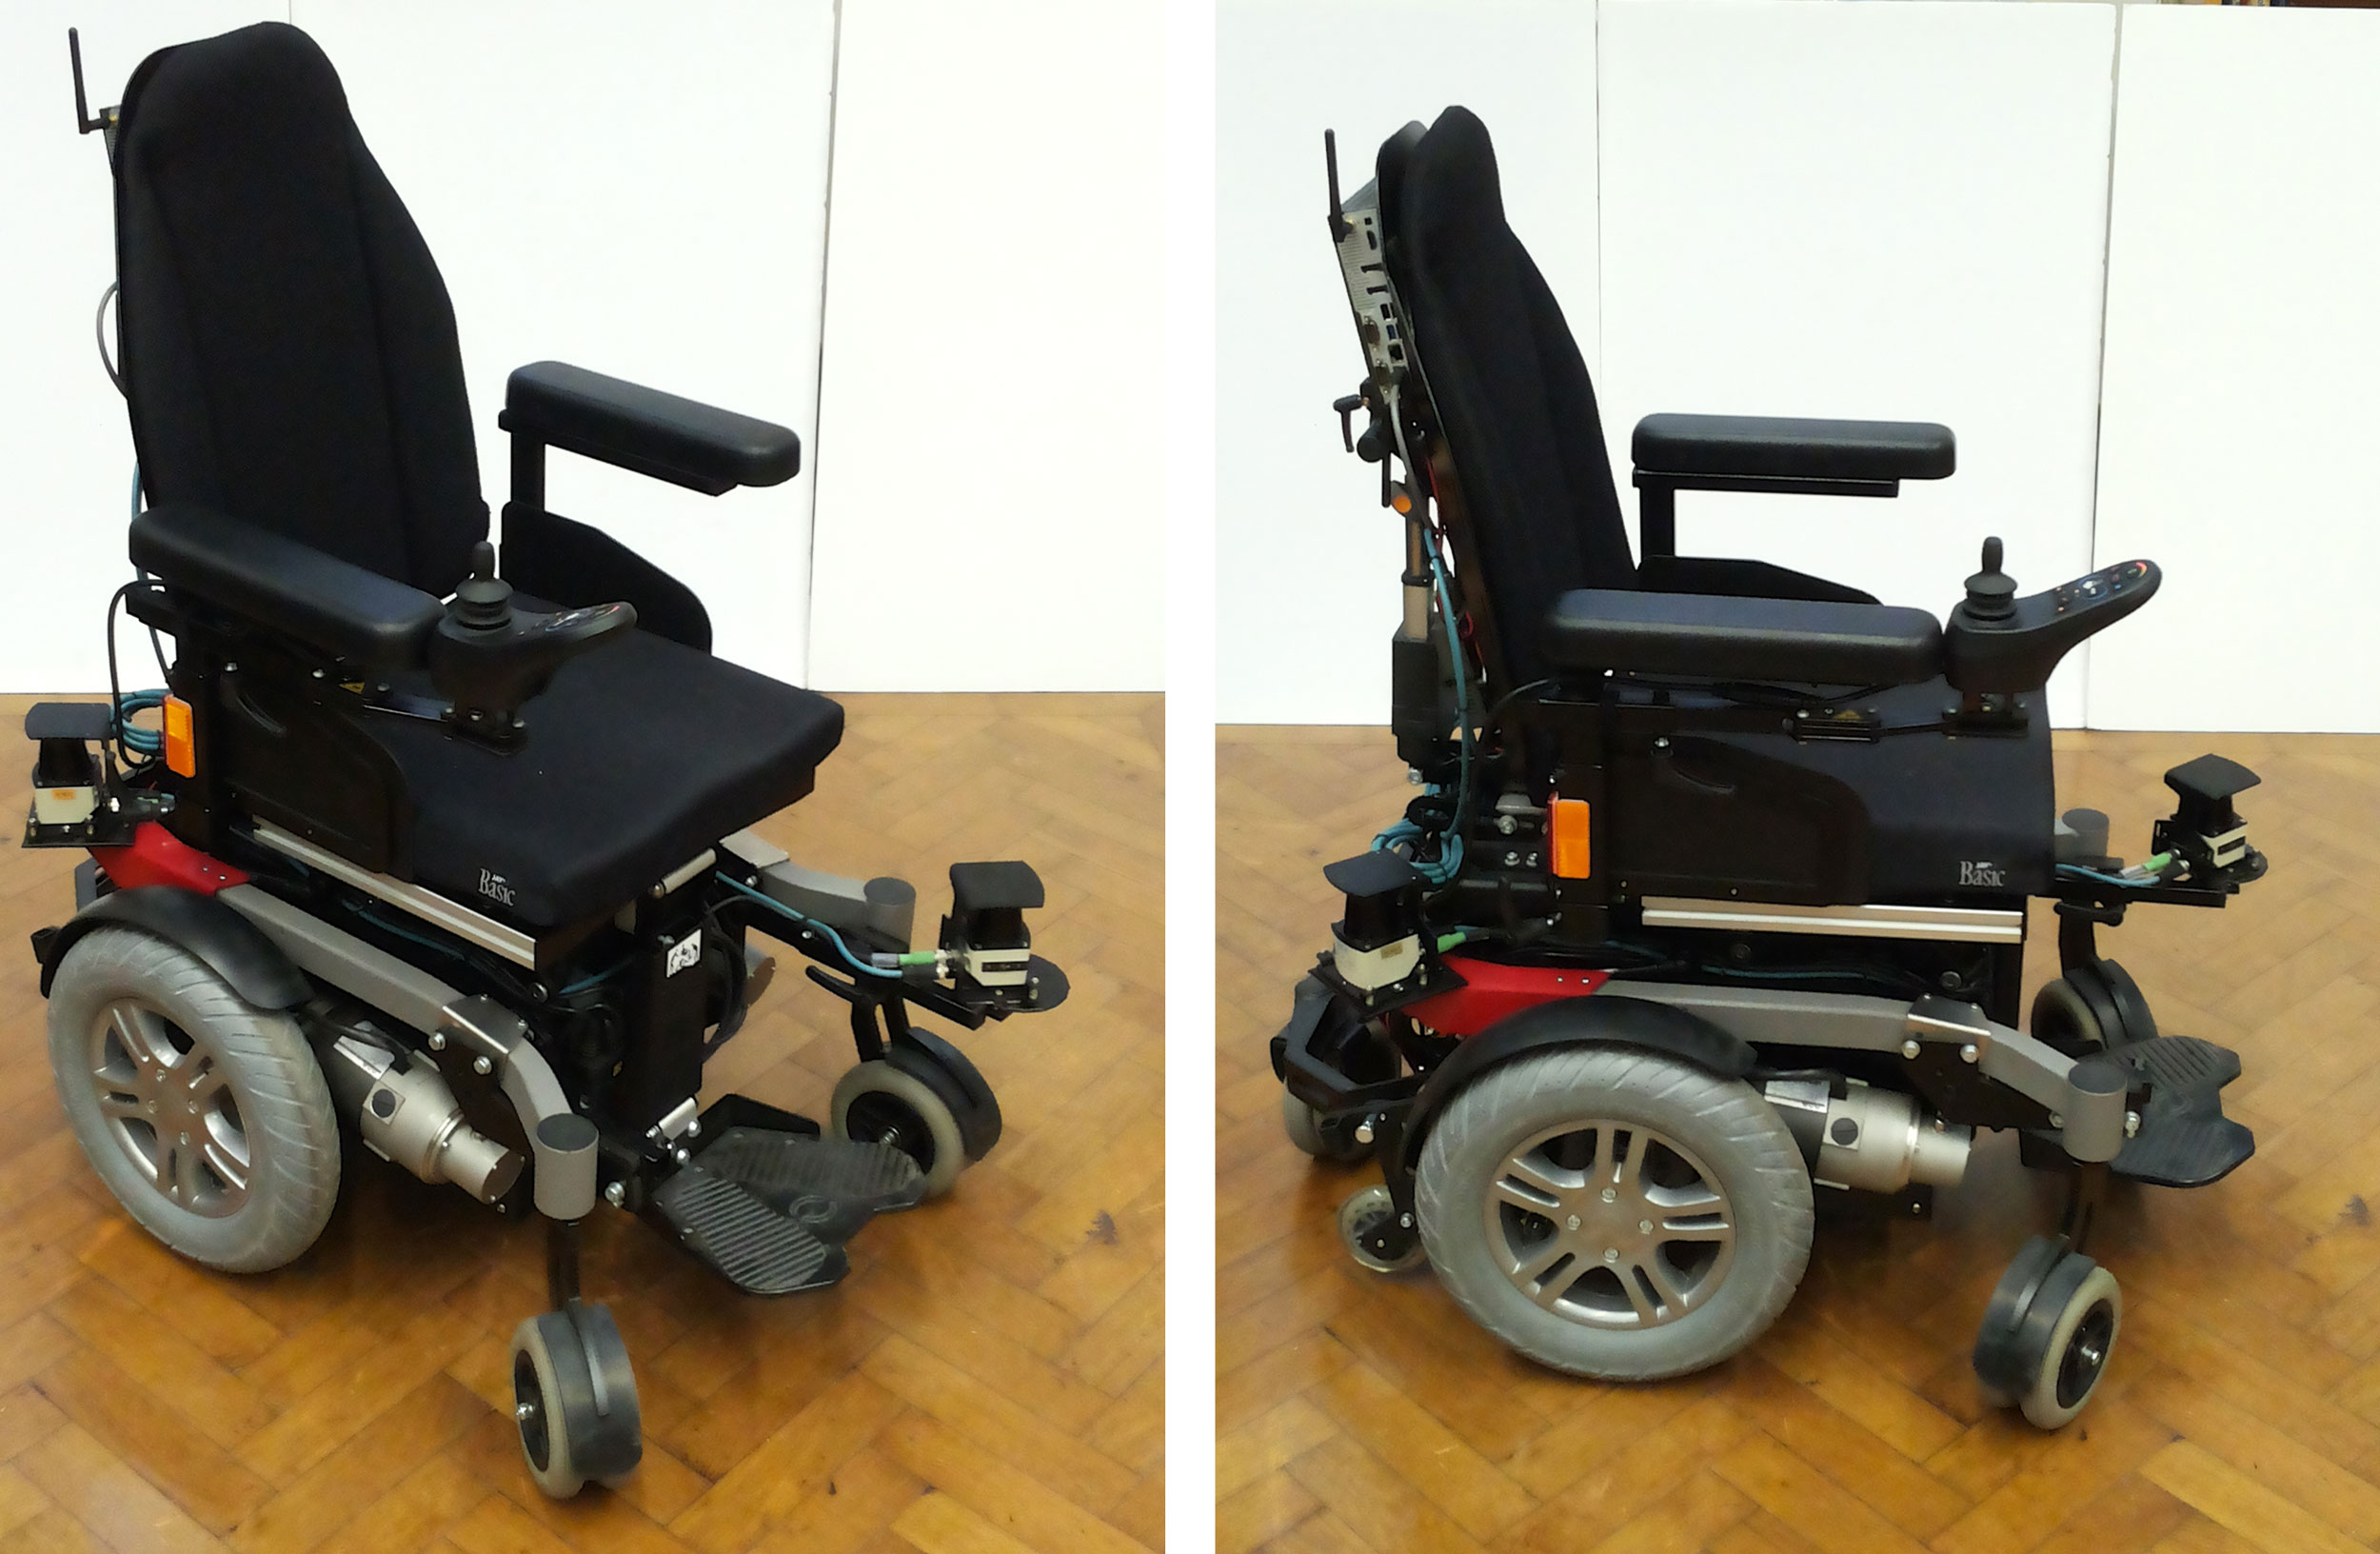
\includegraphics[width=0.95\textwidth]{gfx/pmk/pmk_plat}
\caption{TODO}
\label{fig:pmk}
\end{figure}

\section{The PMK use case}
In this section we give a detailed description of a practical use case where a model-based approach has been used to replicate and reimplement an existing architecture developed with traditional techniques. We decided to start from an already implemented and fully functional system, to show that is possible to achieve the same level of functionalities of the original application with a model-based design combined with automatic programming.

The target robot is an electric wheelchair modified to be controlled with a computer, and equipped with various sensors to achieve levels of autonomy and teleoperation. The wheelchair used as the starting platform is a commercial model (\textit{Twist T4 2x2}) produced by Degonda Rehab SA; it is suitable for both indoor and outdoor usage and it has high manoeuvrability thanks to the two-wheeled dynamics. The conversion from traditional electric wheelchair to autonomous robotic platform is achieved using the Personal Mobility Kit (PMK), which consists in four elements.
\begin{itemize}
\item Encoders connected to the electric motors controlling the wheels, they provide odometry information.
\item Two \textit{Sick TiM 561} laser scanner distance sensors, they provide a 360-degrees coverage around the wheelchair. They are used to map the environment, assist in the localisation of the robot and detect unexpected obstacles.
\item \textit{Shuttle DS81L}, an high-performance slim PC specifically designed for automotive and robotics applications. It is the on-board computer of the robot, it runs ROS and all the application code.
\item The software components necessary to achieve the assisted and autonomous functionalities.
\end{itemize}
The PMK is designed to be an add-on that is possible to mount over any existing electric wheelchair to convert it into an autonomous or semi-autonomous platform. Thus, of the architecture we will present, the only platform specific part is the interface used to interface with on-board electronics, everything else is a modular design that can be adapted to multiple physical platforms.

A commercial electric wheelchair supports manual control through a joystick placed on one of the armrest. While this is suitable for most of users, there are cases of severe disabilities where the patients can only partially or cannot operate the joystick. The objective of PMK is to extend the functionalities of an electric wheelchair to provide assisted and autonomous control. In particular, the implemented software supports four different drive modes.

\paragraph{Manual with PMK off} This is the native configuration of the wheelchair, the user controls the movements directly with the on-board joystick. It is important to maintain the original operational mode even after the modification introduced by the PMK, the electric wheelchair should remain completely functional and operative even if an hardware or software malfunction causes the PMK to stop working. This act as a fallback emergency configuration.
\paragraph{Manual with PMK on} In this configuration the PMK is active, but the user is still completely in control of the wheelchair. When mediated by the software system, the robotic platform can be controlled remotely by using a wireless joypad or directly with the on-board joystick, a priority system ensures that the input from the joystick always has precedence over teleoperation. This is the neutral configuration of PMK, when the system is active, but not performing any action. This mode is particularly useful during the set up phases of the autonomous wheelchair (\eg, environment mapping).
\paragraph{Assisted} In this mode the PMK is enabled and actively meditates the commands coming from any input device. The aim of this configuration is to help the user operate the wheelchair by avoiding obstacles. Set-points sent from the wireless joypad or on-board joystick are processed and, if necessary, modified to avoid obstacle perceived by the two on-board laser scanners. As for the previous mode, the commands coming from the joystick have the priority over the wireless joypad.
\paragraph{Autonomous} Here the wheelchair is fully autonomous, the PMK is in charge of controlling the movements. The user can request a specific goal (\eg, ``take me to the kitchen''), then the robotic platform will automatically reach the destination avoiding any obstacle along the way. For safety reasons, it is always possible to override the commands sent by the PMK in autonomous mode using the on-board joystick.

These are all the main functionalities of the electric wheelchair when equipped with the Personal Mobility Kit. Our aim is to create a system designed and developed using a model-based approach combined with automatic programming that exploits all the problem-related implementations already created for the original architecture and combine them with automatically generated ROS nodes, while maintaining the same functionalities.

\begin{figure}[t]
\centering
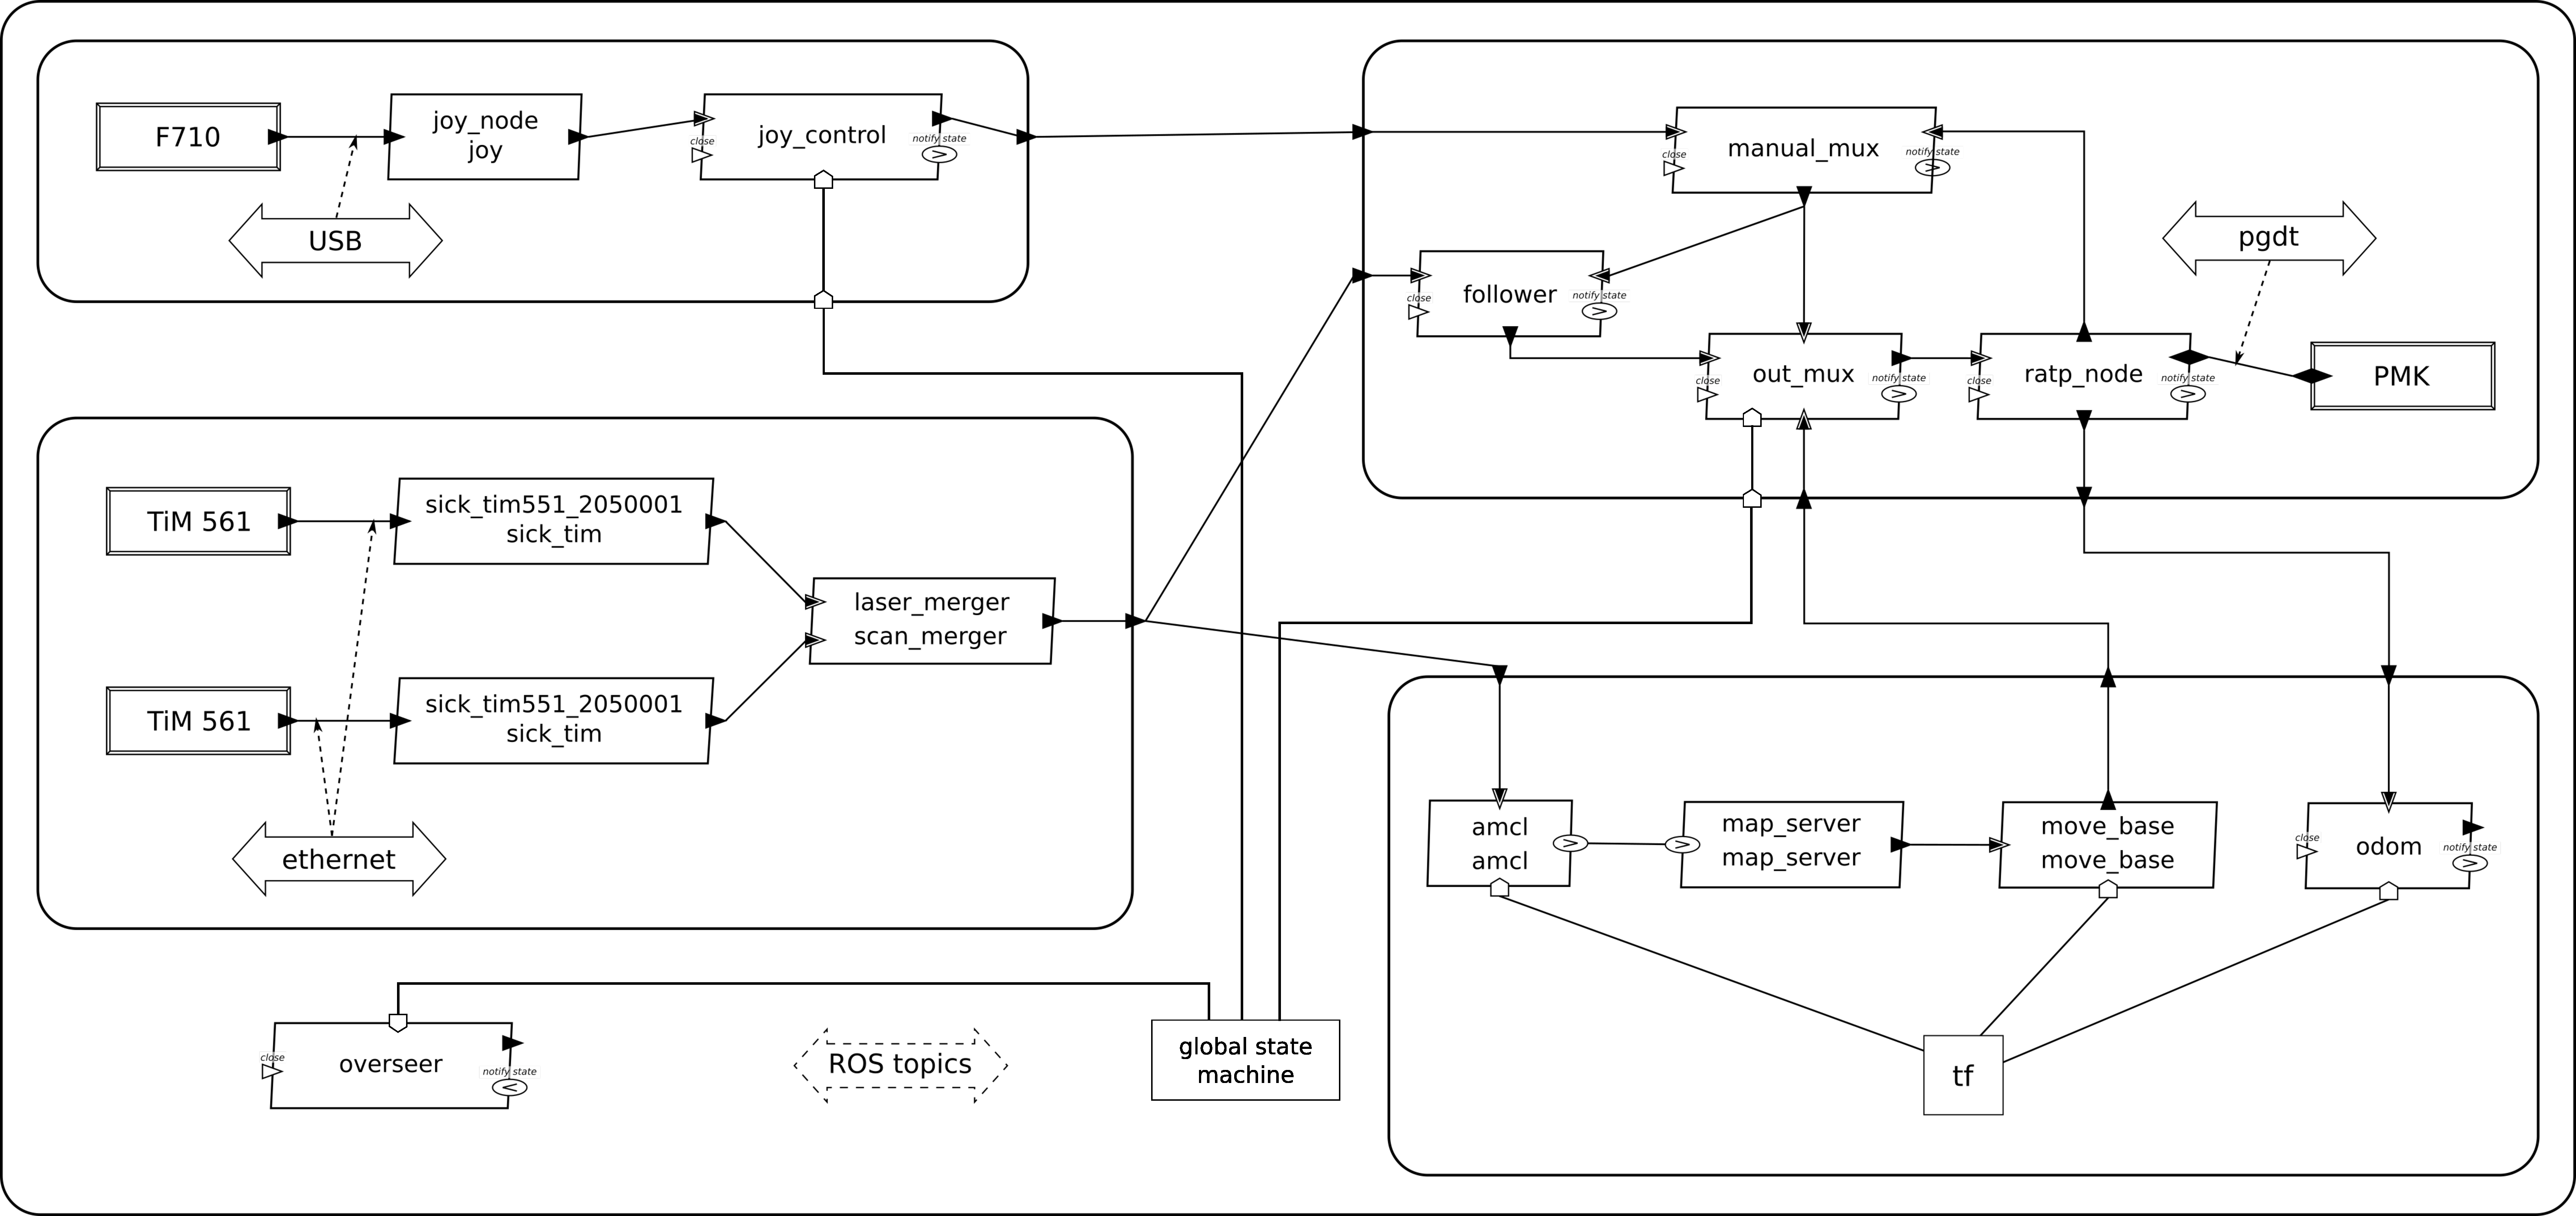
\includegraphics[width=0.95\textwidth]{gfx/pmk/model}
\caption{TODO}
\label{fig:pmk-model}
\end{figure}

\subsection{Model}
The first step of the design of an architecture is to create the model. We did so by following the definitions and meta-models introduced in Chapter~\ref{ch:Modelling}. Figure~\ref{fig:pmk-model} shows a graphical representation of the complete model of the architecture of the robotic wheelchair. To organise and generalise the architecture we exploited the nesting capability of AADL by creating a hierarchical structure of system of systems. Each subsystem capture a specific functionality of the robot, and they are meant to be modular part of the design that can be replaced when necessary. For example, going from laser scanner to cameras, or replacing the navigation system based on \textit{move\_base} with a custom one, or using a different electric wheelchair as platform.

\paragraph{Teleoperation} This subsystem resemble the example presented in Section~\ref{sec:ros-arch}, 

\paragraph{Sensing}

\paragraph{Navigation}

\paragraph{Platform}

\paragraph{Main system}

\subsection{Custom nodes}
Lorem ipsum

\subsection{Special nodes}
Lorem ipsum

\subsection{Comparison}
Lorem ipsum

%*****************************************
